\label{Industrialisation}
JML has the advantage of being a language that can be rapidly and
easily learned and used by developers. One can consider that using a
prover is not so easy. Nevertheless formal activities like modeling
and proving should not be reserved to experts. To demonstrate this
concept, we provide a prover interface understandable to non-experts
in formal methods.

In order to simplify the modeling activity with the JML language, our
interface requirements are:
\begin{itemize}
 \item to be integrated with other tools used by developers, and
 \item not to require the developer to use a mathematical formalism,
    but hide the mathematical formalism under a ``Java'' view.
\end{itemize}
Compared to other formal tools using the JML language, the efforts on
the user interface and integration within the development
environment is probably the main strength of \JACK, as is the fact
that the underlying mathematical formalism is not exposed to the
user.
\paragraph{Integration in developers environment}
 Java developers are used to develop using integrated development
 environments (IDE).  Those IDEs provide many features useful during
 the development process.  Integrating the tool in such IDEs allows
 the user to work in a familiar environment.  This leads both to
 better acceptance of the tool, and to a reduced learning curve.
 Currently, \JACK\ is integrated within the eclipse IDE.  It could
 however be ported to other IDEs, and a standalone version that does
 not require an IDE also exists.

 Another constraint has to be taken into account to obtain developer
 agreement: it is the tool's responsiveness.  The tool has to be used
 interactively, with a debugger spirit: it should not require the
 developer to wait for a long time.  Lemma generation takes, in
 realistic examples, less
 than one minute. %(see Section \ref{Case Study} for metrics).
 Nevertheless, the automatic proof of lemmas is not such a reactive
 activity. Thus, the tool provides a feature that allows to schedule
 proof tasks in order to optimize proof time (see paragraph
 \ref{Support for automatic proof}).


%Several other minor features are available to integrate within the
%development cycle, for example, reports on the status of the project
%can be generated as Microsoft Excel files.
\paragraph{Lemma Viewer}
\begin{figure}[p]
 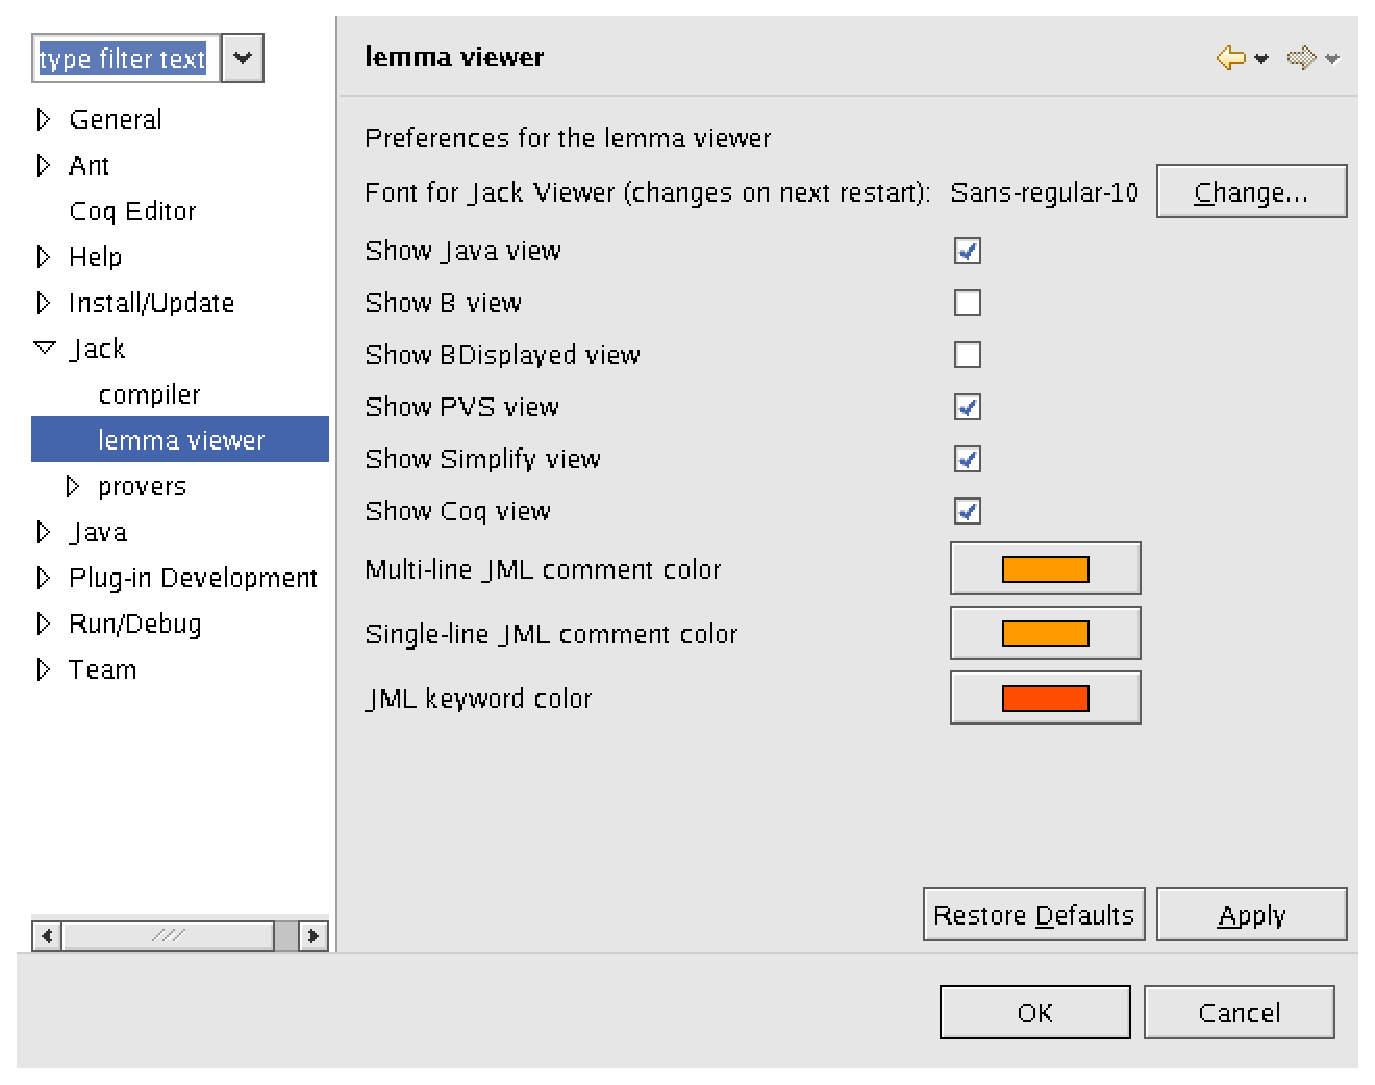
\psfig{file=fm03/preferences-editor.eps,width=14cm}
 \caption{\sc \JACK\ lemma viewer preferences page}
 \label{JACKlemviewprefpage}
\end{figure}
\label{Viewer}
One of the most important points of \JACK\ is that it does not require
developers to learn a mathematical language.  Although lemmas are
generated, those lemmas are not directly displayed to the user.

Instead, we provide the user with a graphical view (Figure \ref{Viewer image}) of the lemma.
 The viewer displays
 \begin{itemize}
  \item information concerning the current proof status;
  \item the class methods with their lemmas;
  \item the source code;
  \item and the currently selected lemma (goals and hypotheses with JPOL and prover language translations).
\end{itemize}
 Within a method, each execution path corresponds to a case.
 Possibly, several lemmas are associated to each case.
 When a case is selected, the corresponding execution path is highlighted.
 When a lemma is selected, its views are displayed.
\subparagraph{Path highlighting}
The source code of the program considered is displayed, and the
path within the program that leads to the generated proof obligation
is highlighted.

\begin{figure}[p]
 \epsfig{file=fm03/jack01.eps,width=15cm}
 \caption{\sc Viewer integrated in eclipse}
 \label{Viewer image}
\end{figure}

Different highlighting colors are used to represent this path:
\begin{itemize}
\item green indicates that the corresponding instruction has been
   executed normally;
\item blue indicates that the corresponding instruction has been
   executed normally, and that additional information is
   available. For instance, the condition of an \texttt{if} construct will
   usually be displayed in blue with additional information indicating
   if the condition has been considered as true or false;
\item red indicates that the corresponding instruction was supposed to
   raise an exception when it has been executed in the case
   considered.  Additional information are also provided indicating
   the exception that has been raised.
\end{itemize}
The part of the specification (invariant or post-condition) that is
involved in the current lemma is also highlighted.  Highlighting the
part of the source code involved in the proof obligation allows to
quickly understand the proof obligation, and allows the user to treat
the proof obligations as execution scenarios of the program.
\subparagraph{Java presentation of lemmas}
The hypothesis and goals of the current lemma are also displayed. As
the conversion mechanism into provers language may be hard to follow, especially by
non-experts, the internal representation used by the tool is used to
present the hypothesis and goals in a Java representation. That is,
all the variables are displayed using the Java dotted notation, and
the Java operators are used instead of their corresponding function.

However, such a translation may be more complicated when operators that
have no Java or JML equivalent constructs are used.  


 However, although the Java view is able to handle some internal
 representation constructs that do not have direct Java or JML
 equivalent constructs, there are still constructs that cannot be
 translated, and for which a Java notation is hard to define. For
 instance some set operators cannot be translated in a generic way.

\subsubsection{Support for verification}
Apart from displaying the generated proof obligations, \JACK\ also
provides support for validating those proofs, as detailed hereafter.
\subparagraph{Support for automatic proof}
\label{Support for automatic proof}
 A point that should not be taken lightly is the time taken by
automatic proof: generating proof obligations for industrial size
applications will generate thousands of proof obligations.

Typically, those proofs can be quite lengthy, and it is necessary that
the user is not obliged to wait for proofs to finish.

To achieve this, \JACK\ provides an independent proof view, where
files can be queued in order to be submitted to the prover. Thus, the
proofs are performed as soon as possible, possibly during the night,
allowing the user to focus on cases inspection.

\subparagraph{Support for interactive proof}
Although the automatic prover allows discharging many proof
obligations, it cannot discharge all the proof obligations. Thus, the
remaining proof obligations have to be verified manually.

Currently, developers are not supposed to handle this task, but to
delegate it to a team of experts that would perform the proofs using
the interactive prover of the \texttt{Atelier B} tool, emacs with PVS
or the Coq editor.


\subparagraph{Checking proof obligations}
Additionally to the ``\textit{proved}'' and ``\textit{unproved}''
states, \JACK\ can also differentiate ``\textit{checked}'' proof
obligations. Checked proof obligations correspond to proof obligations
that are not formally proved, but have been manually verified.

Checking proof obligations is performed by the user to indicate that
he has read and understood the proof obligation and has confidence
that it is correct. Although the checked state provides no formal
guarantee on the correctness of the proof obligations, it still
provides valuable information on the state of a project.

The checked state of the proof obligations can be used in different
ways:
\begin{itemize}
\item To flag cases as already seen in order to start an interactive
   proof only if we are pretty sure that the cases are correct, and
\item In some cases, when a full correctness assurance of the program is not
   required, we may accept that not all the proof obligations are
   formally proved. In that case, it may however, be required that all
   the proof obligations have been checked.
\end{itemize}
In order to minimize verification time, one can assure that checked
proof obligations remain unchanged through subsequents runs of the
proof obligation generator---otherwise the time spent to inspect the
proof obligation and to ensure manually that it is correct would be
lost. 

